\section{系统生物学}
\subsubsection{发展历史}
\begin{frame}
  \frametitle{系统生物学 | 历史}
  \begin{figure}
    \centering
    \includegraphics[width=0.75\textwidth]{c1.introduction/sb.history.01.png}
  \end{figure}
  \vspace{-1em}
    \begin{itemize}
    \item 2000年,第一届国际系统生物学会(1st International Conference on Systems Biology;ICSB 2000)
    \item 2000年,莱诺伊·胡德、阿兰·阿德雷姆及鲁迪·艾伯索尔德,系统生物学研究所(Institute for Systems Biology)
  \end{itemize}
\end{frame}

\begin{frame}
  \frametitle{系统生物学 | 历史 | 分子生物学 vs. 系统生物学}
  \begin{figure}
    \centering
    \includegraphics[width=0.7\textwidth]{c1.introduction/sb.history.02.jpg}
  \end{figure}
  \vspace{-0.8em}
    \begin{block}{Molecular $\Rightarrow$ System}
  Systems biology is a natural extension of molecular biology, and can be defined as ``biology after the identification of key genes".
  \end{block}
\end{frame}

\begin{frame}
  \frametitle{系统生物学 | 历史 | 组学 $\rightarrow$ 系统生物学}
  \begin{figure}
    \centering
    \includegraphics[width=0.9\textwidth]{c1.introduction/sb.history.05.jpg}
  \end{figure}
\end{frame}

\subsubsection{学科定义}
\begin{frame}
  \frametitle{系统生物学 | 定义}
  \begin{block}{莱诺伊·胡德,2001}
    系统生物学是将DNA、RNA、蛋白质以及三者彼此之间的交互作用等信息加以整合,并运用这些资料去建立出数学计量模型,以期能掌握所有生物基因与组织间的关系及运作。\\
  \end{block}
  \pause
  \begin{block}{Hood,2004}
系统生物学是研究一个生物系统中所有组成成分(基因、mRNA、蛋白质等)的构成,以及在特定条件下这些组分间的相互关系,并通过计算生物学建立一个数学模型来定量描述和预测生物功能、表型和行为的学科。
  \end{block}
  \pause
  \begin{block}{杨胜利,2004}
系统生物学是在细胞、组织、器官和生物体水平上研究结构和功能各异的生物分子及其相互作用,并通过计算生物学定量阐明和预测生物功能、表型和行为。系统生物学将在基因组测序基础上完成DNA序列到生命的过程,这是逐步整合、优化的过程,系统生物学的发展预计需要一个世纪或更长的时期,因此常把系统生物学称为21世纪的生物学。
  \end{block}
\end{frame}

\begin{frame}
  \frametitle{系统生物学 | 定义}
  \begin{figure}
    \centering
    \includegraphics[width=0.6\textwidth]{c1.introduction/sb.01.jpg}
  \end{figure}
\end{frame}

\subsubsection{研究内容}
\begin{frame}
  \frametitle{系统生物学 | 内容}
  \begin{block}{湿实验}
采用高通量实验技术,通过众多组学,在整体和动态研究水平上积累数据并在挖掘数据时发现新规律、新知识,提出新概念。
  \end{block}
  \pause
  \begin{block}{干实验}
通过计算生物学建立生物模型,根据被研究的真实系统的模型,利用计算机进行实验研究。
  \end{block}
\end{frame}

\begin{frame}
  \frametitle{系统生物学 | 内容}
  \begin{figure}
    \centering
    \includegraphics[width=0.8\textwidth]{c1.introduction/sb.content.03.png}
  \end{figure}
\end{frame}

\subsubsection{工作流程}
\begin{frame}
  \frametitle{系统生物学 | 流程}
  \begin{columns}
    \column{0.35\textwidth}
    \begin{block}{流程}
  \begin{enumerate}
    \item 研究组分,构建模型
    \item 改变条件,观测变化
    \item 比较结果,修订模型
    \item 重新实验,继续修订
  \end{enumerate}
    \end{block}
    \column{0.65\textwidth}
  \begin{figure}
    \centering
    \includegraphics[width=0.9\textwidth]{c1.introduction/sb.workflow.03.png}
  \end{figure}
  \end{columns}
\end{frame}

\subsubsection{研究方法}
\begin{frame}
  \frametitle{系统生物学 | 方法 | 整合与干涉}
  \begin{block}{整合(incorporation)}
把系统内不同性质的构成要素(DNA、RNA、蛋白质和生物小分子等)或不同层次的构成要素整合在一起进行研究。
  \end{block}
  \pause
  \begin{block}{干涉(perturbation)}
人为地设定某种或某些条件去作用于被实验的对象,从而研究特定的生命系统在不同时间和空间条件下具有的动力学特征。
  \end{block}
\end{frame}

\begin{frame}
  \frametitle{系统生物学 | 方法 | 整合与干涉 | 整合策略}
  \begin{columns}
    \column{0.45\textwidth}
    \begin{itemize}
    \item 自下而上(hypothesis based):使用独立的实验数据,适用于大多数基因和它们的调控关系相对比较清楚的情况
    \item 自上而下(data driven):利用高通量的DNA芯片和其他新的测试技术获得数据来研究
    \item 混合使用:自下而上 + 自上而下
  \end{itemize}
    \column{0.55\textwidth}
  \begin{figure}
    \centering
    \includegraphics[width=0.9\textwidth]{c1.introduction/sb.tdbu.01.jpg}
  \end{figure}
  \end{columns}
\end{frame}

\begin{frame}
  \frametitle{系统生物学 | 方法 | 建模和模拟}
  \begin{figure}
    \centering
    \includegraphics[width=0.65\textwidth]{c1.introduction/sb.model.01.jpg}
    \includegraphics[width=0.33\textwidth]{c1.introduction/sb.simulation.01.png}
  \end{figure}
\end{frame}

\subsubsection{应用前景}
\begin{frame}
  \frametitle{系统生物学 | 应用}
  \begin{figure}
    \centering
    \includegraphics[width=0.9\textwidth]{c1.introduction/sb.application.01.jpg}
  \end{figure}
\end{frame}

\begin{frame}
  \frametitle{系统生物学 | 应用}
  \begin{figure}
    \centering
    \includegraphics[width=0.55\textwidth]{c1.introduction/sb.application.02.png}
    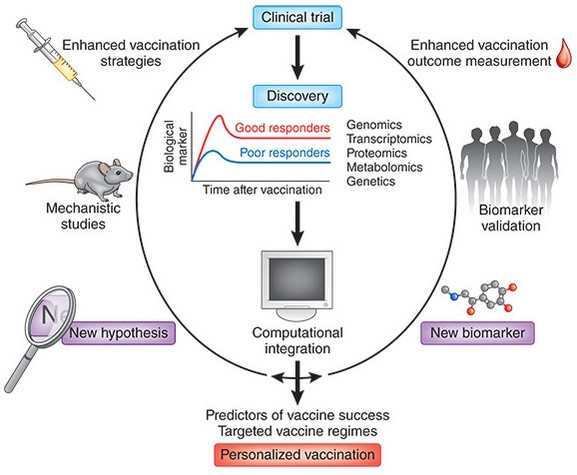
\includegraphics[width=0.42\textwidth]{c1.introduction/sb.application.04.jpg}
  \end{figure}
\end{frame}

\begin{frame}
  \frametitle{系统生物学 | 前景}
  \begin{figure}
    \centering
    \includegraphics[width=0.6\textwidth]{c1.introduction/sb.future.01.jpg}
  \end{figure}
\end{frame}
